% !TEX root = ../thesis.tex

\chapter{Theory}
\label{chap:theory}

\cleanchapterquote{At the end of the century one will be able to speak of machines thinking without expecting to be contradicted.}{Alan Turing}{(Computing Machinery and Intelligence in 1950)}


% ------------------------------------------------------------------------------

In this chapter, I cover the basic concepts of neural networks that will be used later on when separation of style and content is discussed in more detail.
My intention is to allow anybody with basic knowledge in Mathematics and Computing to understand this manuscript from beginning to end.

The explanations will be developed from basic to complex so that sequential reading should guide the reader logically from question to answer while giving as much insight as will be necessary to continue and just enough context to understand the raison d'être of the each concept.


% ------------------------------------------------------------------------------

\section{Background}
\label{sec:theory:background}

Before diving into technical aspects, however, I believe it is worth stopping first to introduce the main areas of this research: \emph{Neural Networks} and \emph{Deep Learning}.
Neural Networks is an area of \emph{Machine Learning} very closely related with \emph{Cognitive Sciences} and Deep Learning is also an area of Machine Learning that typically uses neural networks, but let us go step by step.


\subsection{Neural Networks}
\label{sub:theory:background:neural-networks}

We can describe the field of Machine Learning as the study that enables computers to resolve problems for which they have not been explicitly programmed for by using some learning mechanism, as \citet{Samuel1959} postulated.
When explicitly programming an algorithm to resolve a problem, its complexity grows dramatically with that of the problem and the desired precision.
A perfectly robust algorithm that follows this approach will require: 1) the programmer to understand the problem completely so that all variables can be taken into account; 2) a hardware powerful enough to handle all these variables; and 3) data with maximum precision.
It is easy to see how one or more of these requirements will pose complications when the problem is complex enough.
Driving a car is a complex enough problem to make classic computing incapable of solving it.
Conversely, driving a car is a simple enough problem so that any person can do it.
The human mind can handle the task because, although not having perfect senses nor 100\% understanding of the laws of physics, how the car works, how other drivers exactly behave, and many other factors involved; it is capable of dealing with partial information, uncertainty, imprecision, and approximations after having learned from experience \cite{Zadeh1994}.
In contrast to how classic computing tries to accurately model the world to solve problems, some fields of Machine Learning try to model how the human mind learns the complexity of the world to reason and act upon it.

At this point, it is clear how the study of the human mind plays an important role in machine learning.
Cognitive sciences is the field that studies the human mind and how it acquires understanding through experience and the senses.
Modern cognitive sciences originated in the 1940s, when efforts were being made to understand the principles of the mind by representing their structures and processes instead of operating directly on them \cite{Thagard2008}.
The studies quickly branched off in 1943 when \citet{McCulloch1943}, inspired by biological neural networks, described the first mathematical model of an artificial neural network.
The field of Neural Networks, shorthand for \emph{Artificial Neural Networks} (ANNs), quickly grew in the 1950s when they started being implemented \cite{Farley1954,Rosenblatt1958}.

Since then, the field has evolved and expanded into a myriad of different methods, maintaining the similarity with their biological counterparts in greater or lesser degree.
Within the general framework, we can still talk of neurons organized in \emph{layers}, implementing an \emph{activation function}, and storing experience in \emph{weights}, as depicted in Figure~\ref{fig:sec:theory:neurons}.
An artificial neuron is a simple processing unit, forming networks typically organized in layers, whose input is the set of outputs of connected neurons from the previous layer and where the process it performs is determined by the activation function.
The activation function can be implemented either as a threshold to be reached for the neuron to send an output or simply as a transformation of any sort of the input.
Lastly, experience in ANNs can be understood as connection strength between neurons in biological neural networks and this mechanism is implemented as a set of learnable parameters, commonly called weights, that modify the value of each input to the neuron \cite{Hinton1989}.

\begin{figure}[t]
  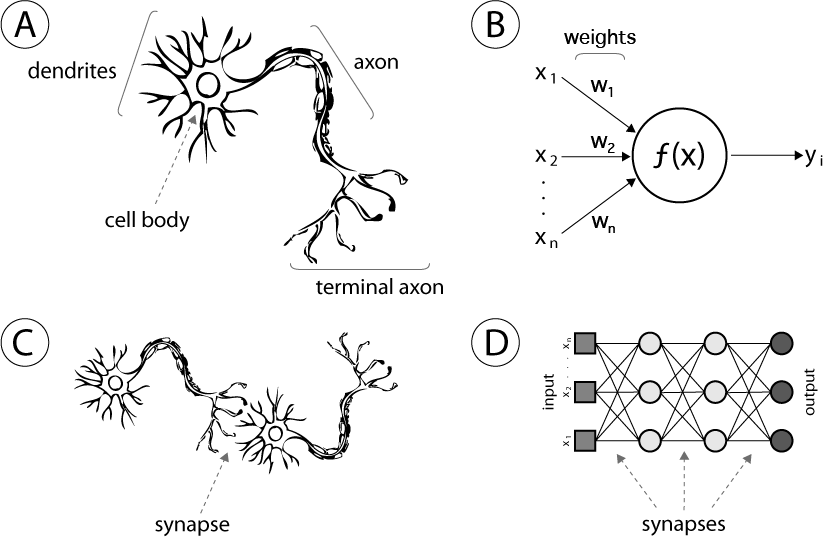
\includegraphics[width=\textwidth]{gfx/neurons}
  \caption{
    Biological Neuron vs. Artificial Neuron \cite{Honorio2013}.
    AC) A biological neuron receives signals at the dendrites, the composition of the signals may or may not produce an excitation in the cell body based on experience, in which case a pulse will be transmitted down the axon and ultimately to other neurons' dendrites via terminal axon in a process called synapsis.
    BD) Similarly, artificial neuronal networks are organized in layers and synapses occur from layer to layer.
    An artificial neuron in the layer $Y$ receives one or more inputs $X$, representing dendrites, and as a result of an activation function $f(X)$ produces an output $y_i$, representing the axon, that gets passed to connected neurons in the subsequent layer.
    Weights represent the connection strength between neurons and encode network experience.
  }
  \label{fig:sec:theory:neurons}
\end{figure}

A crucial step in preparing an ANN for a specific task is refining its set of weights.
That is what we refer to as training or supervised learning process.
Supervised learning is a data-driven process that requires a labeled training set of examples of which we know their class (e.g. dog vs. cat).
The process can be implemented in several ways but it generally boils down to defining some way to assess how far the prediction of the network is away from an optimal solution, an estimate given by a \emph{loss function}, and the strategy that will propagate the error as well as refine the weights of the network.
Eventually, after enough training examples and corrections, the weights of the network will have adapted to generalize the features of the training data and will be more or less able to correctly classify new incoming examples.

The process can be seen as a teacher supervising the learning of a student.
The ``teacher" (loss function + weight rectification strategy) knows the correct solution (label of the example) and it corrects the ``student" (the network) when its prediction is incorrect.
An example of a completely wrong prediction would be the network having 100\% confidence of an image containing a dog when it clearly contains a cat.

One of the most important aspects that determine the accuracy of the network when presented with new examples is the volume of data and the correctness of its labels.
This becomes extremely important when trying to solve real-world problems like image recognition, where massive training sets are required to generalize networks for all concepts in a language under several different lighting conditions.
Big enough volumes of data have not been readily available until recently, and even nowadays, complete and accurately labeled datasets are expensive or time consuming to handcraft as the task may be too large or require expert knowledge on the specific field.
One approach to work around this is semi-supervised learning, using partially labeled training datasets and pre-training the network first with unsupervised training, where unlabeled examples are employed so that the network learns how to identify recurring patterns, which are later employed to improve the performance of the supervised learning process \cite{Zhu2008}.
Reducing the number of weights the network requires to correctly classify the input is another complementary solution that has seen much success lately and it is one of the recurring features of many deep learning techniques.


\subsection{Deep Learning}
\label{sub:theory:background:deep-learning}

Since 2006, the field of \emph{Deep Learning}, also called hierarchical learning, has appeared as a new area of Machine Learning research that brings it closer to its original goals: Artificial Intelligence \cite{Deng2014}.
Deep learning focuses its efforts on producing methods for learning hierarchical feature representations, different levels of abstraction where higher-level ones are defined from lower-level ones, helping to make sense of data such as images, sound, and text in real-world applications.

One clear example of hierarchical representation is a spoken sentence.
A spoken sentence, the higher-level concept, is composed of spoken words.
A spoken word is made up of phonemes.
A phoneme is a representation of a speech sound with an associated waveform.
Making sense of speech in deep learning means first analyzing the waveform looking for phonemes, then trying to make up words from the phonemes found, and finally producing a grammatically correct and semantically meaningful sentence with those words.

As already mentioned in Chapter~\ref{chap:intro}, this kind of pattern recognition did not perform well until recently.
Traditional solutions employed shallow neural networks with simplistic models and limited representation power that could only be used to solve well-constrained problems like numerical approximations or binary classification.
Speech recognition, contrarily, is a very loosely-constrained problem and that is also the case for any problem dealing with the richness of data such as human voice, natural language, and natural images.

Studies in human information processing mechanisms suggested the human brain uses deep neuronal architectures to extract complex patterns and build internal representations from rich sensory inputs.
For instance, the human speech perception system in the brain is equipped with layered hierarchical structures that transform the information from the acoustic level to the linguistic level \cite{Deng1999,Baker2009}.
Training analogous deep architectures in artificial neural networks, \emph{deep neural networks} (DNNs), proved problematic from the beginning since classic learning algorithms tended to quickly get stuck in local optima and produced inaccurate classifications.
This phenomenon, unfortunately, worsened quickly the more layers the neural network presented, which is the case of DNNs.

Efficient unsupervised learning algorithms that made use of increasingly big datasets, available thanks to the widespread use of the Internet, were proposed to overcome the problems presented by local optima in classic learning algorithms \cite{Bottou2004,Hinton2006}, as previously discussed in Section~\ref{sub:theory:background:neural-networks}.
They, however, were so computationally expensive for training deep neural networks, having millions of parameters to learn, that were not widely used until parallelizable variations were proposed \cite{Dean2012,Chen2012}.
Powerful Graphic Processing Units (GPUs) becoming a commodity finally allowed quick implementations of these algorithms and marked the rapid development of deep learning in recent years.

Deep Learning is at the moment a quickly growing field covering a wide range of machine learning techniques and architectures.
In this research, we cover only the architecture of DNNs that we need for further discussing the separation of style and content, \emph{convolutional neural networks} in Section~\ref{sec:theory:convnets}.
Before jumping too far ahead, the next sections of this chapter will go through the evolution of relevant ANNs architectures down from the most basic one, the \emph{perceptron}, up to the one at hand, convolutional neural networks.


% ------------------------------------------------------------------------------

\section{Perceptron}
\label{sec:theory:perceptron}

The perceptron was the first ever implemented neural network.
It was created by \citet{Rosenblatt1958} in 1957 based on the studies of \citet{McCulloch1943} and it featured the simplest architecture possible in an ANN, composed of a single neuron.

The perceptron can be described as performing a task of binary classification, which is simply deciding which of two mutually exclusive classes a set of inputs belongs to \cite{Freund1999} and it is mathematically expressed as follows:

$$
  f(x) =
  \begin{cases}
    1 & \text{if } {w}\cdot{x}+b > 0\\
    0 & \text{otherwise}
  \end{cases}
$$

Where $x$, an array of real values, represents the input of the perceptron; $w$, also an array of real values, represents the weights; $b$ is the \emph{bias}; ${w}\cdot{x}$ is the dot product; ${w}\cdot{x}+b > 0$ is the activation function; and, finally, $0$ and $1$ correspond to the mutually exclusive classes.

The inputs are visualized as data points in the space of variables and the activation function as a linear boundary that leaves them classified either above or below it.
The weights are used to measure the relevance of each one of the inputs in the final classification, parameters that get learned during the training process in the same fashion as I described in Section~\ref{sub:theory:background:neural-networks}.
The bias gets also learned during the training process, but it does not depend on any input value and is used to control the position of the linear boundary.
The dot product can also be expressed as a weighted sum $\sum_{i=0}^{m} w_i x_i$ where $m$ is the number of parameters the perceptron receives per input, as it is depicted in Figure~\ref{fig:sec:theory:perceptron}.

\begin{figure}[t]
  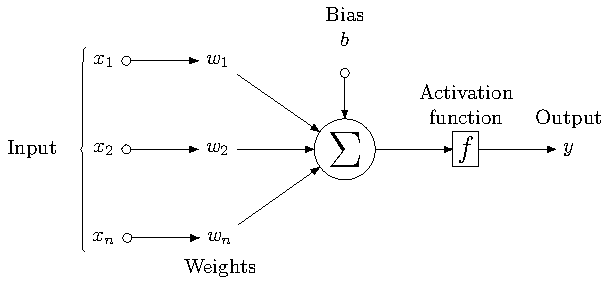
\includegraphics[width=\textwidth]{tkz/perceptron}
  \caption{
    Anatomy of the Perceptron \cite{Medina2013}.
    In the center, represented by $\sum$, there is the weighted sum of inputs.
    Mathematically expressed as the dot product (${w}\cdot{x}$) of the vector of inputs $x$ with the vector of weights $w$, both containing real values.
    The activation function triggers a binary output $y$ if ${w}\cdot{x}$ plus the bias $b$, also a real value, is above $0$.
  }
  \label{fig:sec:theory:perceptron}
\end{figure}

Perceptrons can be trained with supervised learning for trying to find the weights in the binary classifier function to correctly classify some training dataset.
Let us imagine we want to train a perceptron to classify animals into either cat or dog based on their size and level of domestication.
Our training data is labeled, meaning that for each pair $(size, domestication)$ we know whom it actually belongs to, either a cat or a dog.
We start with a perceptron whose weights are set to random values and the first training example gets classified randomly.
As new training examples arrive, the learning algorithm will update the weights of the perceptron so that the linear boundary described by ${w}\cdot{x}+b$, the activation function, leaves data points correctly classified in both sides.
Figure~\ref{fig:sec:theory:perceptron-training} depicts how this process happens.

\begin{figure}[t]
  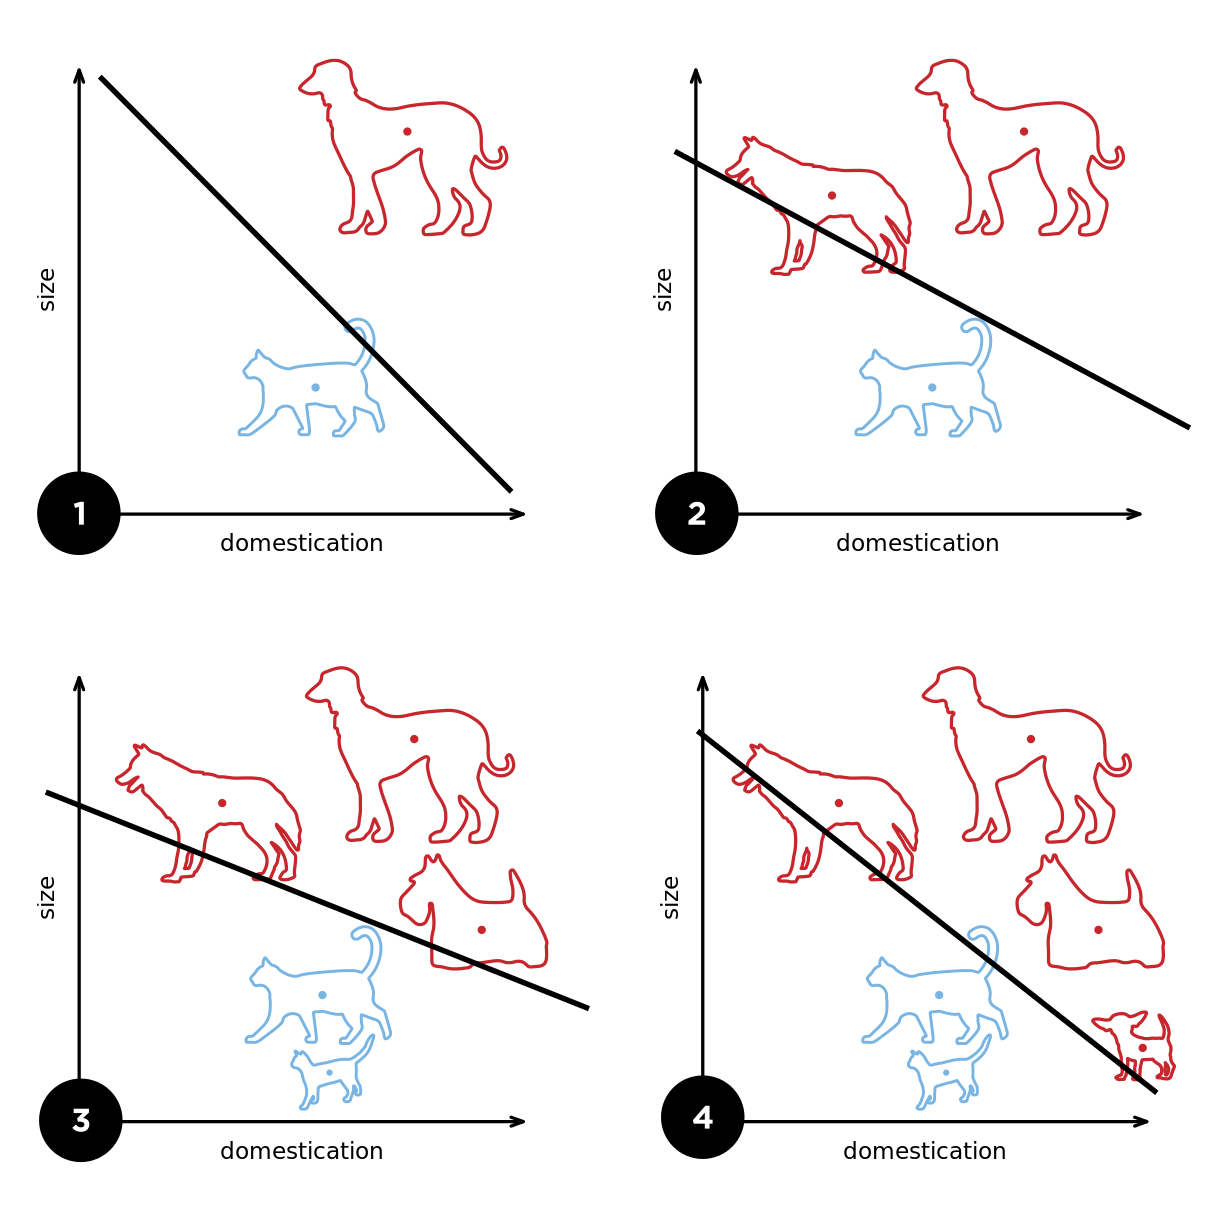
\includegraphics[width=\textwidth]{gfx/perceptron-training}
  \caption{
    Linear boundary of a perceptron adjusting to new training examples \cite{Goodspeed2015}.
    The perceptron classifies inputs with two variables: $size$ and $domestication$, into two classes, dog or cat.
    Supervised learning adjusts the linear boundary to accommodate the new data points into their correct category.
  }
  \label{fig:sec:theory:perceptron-training}
\end{figure}

The main problem with the perceptron is that the training will never converge to a set of weights that correctly classify the training examples if these are not linearly separable, and thus predictions of new data points will consistently be wrong.
These limitations were mathematically proved by \citet{Minsky1969} in 1969.
Not only that, they also claimed perceptrons with multiple layers of neurons would not be capable of overcoming non-linearities, leading to believe that neural networks would not be feasible for scalable intelligent systems and managing to discourage further efforts in the field for over a decade.
Little to none research was done in the field until \emph{backpropagation}, a learning algorithm for \emph{multi-layer neural networks}, was developed by \citet{Werbos1974}, rediscovered by \citet{Parker1985}, and finally popularized by \citet{Rumelhart1986} in the 1980s \cite{Ruck1990}.
The efficient use of multi-layer feedforward neural networks marked the rise in popularity of the field.


% ------------------------------------------------------------------------------

\section{Multi-layer Feedforward Neural Networks}
\label{sec:theory:mlffnn}

While introducing the perceptron, we could not really speak of it as neural network per se, since we were discussing an architecture consisting of a single neuron.
We introduce now multi-layer feedforward neural networks, composed of several layers of neurons, them being fully connected with the neurons of the adjacent layers and data always flowing forward.
Figure~\ref{fig:sec:theory:mlffnn} depicts such \emph{feed-forward} architecture where data flows, represented as arrows, never forms a cycle, opposed to other more complicated types of architectures where data is fed back to previous layers.
These networks behave like we described when talking about the perceptron both in their first layer, representing the parameters of the input, and in their final layer, performing classification.
Intermediate layers, called \emph{hidden layers}, are the most interesting addition to the architecture.
Neurons in them perform intermediate predictions and these are fed to neurons in the next layer.
The fully-connected architecture architecture allows for different neurons in the hidden layers to make predictions of different patterns in the raw input and letting neurons in subsequent layers predict based on those patterns instead.

If we zoomed in on one the nodes we would see replicated exactly the same structure as we presented previously for the perceptron in \autoref{fig:sec:theory:perceptron}.
Inputs get weighted and summed, and the result of that passed to some function that performs the prediction.
One important difference to note is that for the input of subsequent layers to still be real values, neurons in hidden layers must implement non-linear activation functions, representing the probability or certainty of the example belonging to a class.
Non-linear activation functions are also normally called \emph{transformation functions} since they transform the input rather than producing a binary classification.
Non-linearities often used are the hyperbolic tangent, $\tanh(x)$, or the logistic function, $(1+e^{-x})^{-1}$, which are inspired by biological neurons' \emph{action potential}, and allow for non-linear classification \cite{Thorpe1989}.

Unlike the perceptron and contrary to incorrect beliefs induced by a misinterpretation of \citeauthor{Minsky1969}'s analysis of the perceptron limitations, disproved by \citet{Hornik1989} in 1989, multi-layer feedforward networks with at least one hidden layer are capable of making predictions of arbitrary precision given enough data regardless of it being non-linearly separable.
These networks' capabilities make of them universal approximators and viable for intelligent systems, being the key for such an achievement backpropagation, a general purpose supervised learning algorithm for feed-forward networks \cite{Rumelhart1986}.

\begin{figure}[t]
  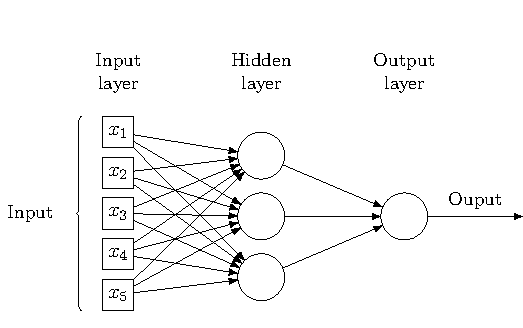
\includegraphics[width=\textwidth]{tkz/mlffnn}
  \caption{
    Architecture of the most simple multi-layer neural network \cite{Medina2013A}.
    The first layer, at the left, represents the parameters of the input that get fed into each one of the neurons of the next layer.
    The last layer, at the right, performs the final classification.
    The layers in between, called hidden layers, also perform intermediate classification and their output is fed as input to the next layer.
  }
  \label{fig:sec:theory:mlffnn}
\end{figure}


\subsection{Backpropagation}
\label{sec:theory:mlffnn:backpropagation}

Training single-layer networks, where the input is directly connected to the output layer, is relatively simple.
As we described before, it only requires iteratively adjusting the weights to correctly classify the training examples based solely on the input parameters.
Training multi-layered networks becomes much more difficult since the final prediction is not directly related to the original input parameters, but to all intermediate predictions in hidden layers and thus to their weights as well.
Consequently, a learning procedure for these networks should determine the weights of neurons in hidden layers that will result in the intermediate predictions that will produce correct predictions at the output of the network.
This is equivalent to making the neurons in hidden layers learn internal representations of incoming data, which is one of the main interests of using multi-layered networks to solve real-world problems that are hard to model, be it due to lack of knowledge in the domain or to the complexity of the task.

Learning in neural networks can be generally approached as an optimization problem.
For each training example $(x, t)$, being $x$ the array of input parameters, we first must find the minima in the error function, e.g. $E = (t - y)^2$, being $t$ the correct prediction, also referred to \emph{ground truth}, and $y$ the prediction of the network.
At the same time, $y$ is a function representing the operation performed by the network as a whole, depending on the weights $w$ that will ultimately be adjusted to minimize the error $E$.

\autoref{fig:sec:theory:mlffnn:error-function} shows the visual representation of the error function for a single-layer neural network with 2-parameter inputs, being $y = w_1 x_1 + w_2 x_2$, the transformation function.
There are several methods to find the minima of such parabolic function, but \emph{gradient descent} is normally used.
In multi-layered networks, on the other hand, $y$ is a composite function of increasingly nested transformation functions on each layer.
For a network, $y$ would be $\sum_i w_i f_i(x)$, being $i$ neurons of the last hidden layer, $w_i$ the weight assigned to their output, and $f_i$ their transformation function, described by $\sum_j w_j f_j(x)$, being $j$ neurons of the previous hidden layer.
This continues until the first hidden layer.
Gradient descent can be efficiently applied on this kind of chained functions using the chain rule, as described by \citet{Linnainmaa1976} and implemented in the backpropagation algorithm.

\begin{figure}[t]
  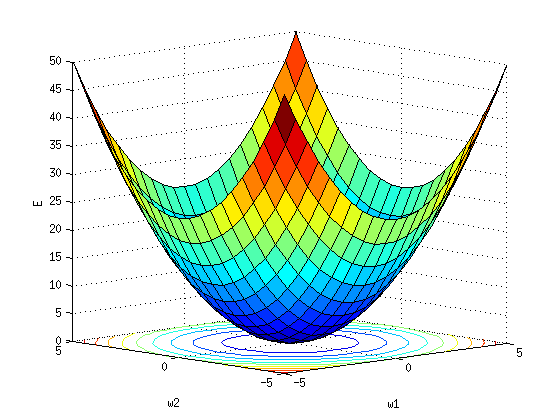
\includegraphics[width=\textwidth]{gfx/error-function}
  \caption{
    Error function of a single-layer neural network with two input weights \cite{AI4562013}.
    The function is defined by $E = (t - (w_1 x_1 + w_2 x_2))^2$ and finds its minima at $E = 0$ when $w_1$ and $w_2$ correctly predict $t$ for the input $x$.
  }
  \label{fig:sec:theory:mlffnn:error-function}
\end{figure}

Backpropagation, inspired on the mathematical intuition, describes an approach for adjusting the weights of the whole network based only on the output prediction error and scales up for arbitrarily big networks by propagating the error and correcting weights locally for each neuron.
The algorithm consists of two phases: 1) error propagation, and 2) weight correction.

During error propagation, for a training example, the algorithm first calculates the error $E$ for the prediction $y$ in the output layer.
The error gets then propagated backwardly to all neurons layer by layer, as represented in \autoref{fig:sec:theory:mlffnn:backprop-1}.
The propagated error for a neuron $i$ within a given hidden layer is calculated as $E_{i} = \sum_j w_{ij} E_{j}$, being $j$ a neuron in the following layer (closer to output), $E_{j}$ its calculated error, and $w_{ij}$ its associated weight for neuron $i$.
Propagated errors represent how much of the overall error was contributed by the neuron on its layer.

\begin{figure}[t]
  \begin{subfigure}[b]{0.5\textwidth}
    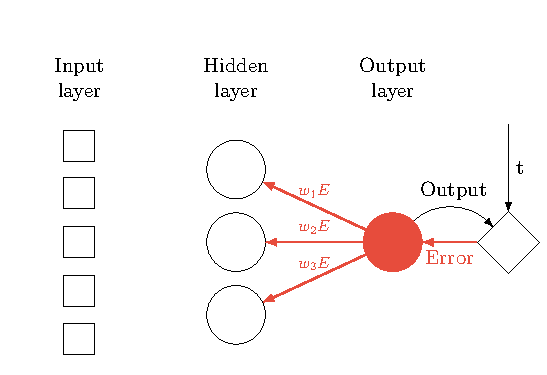
\includegraphics[width=\textwidth]{tkz/mlffnn-backpropagation-1}
    \caption{Error propagation}
    \label{fig:sec:theory:mlffnn:backprop-1}
  \end{subfigure}
  \hfill
  \begin{subfigure}[b]{0.5\textwidth}
    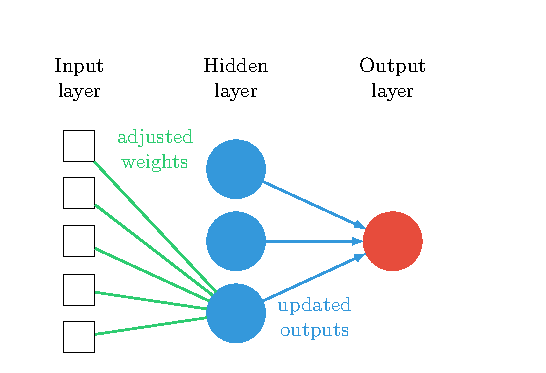
\includegraphics[width=\textwidth]{tkz/mlffnn-backpropagation-2}
    \caption{Weight correction}
    \label{fig:sec:theory:mlffnn:backprop-2}
  \end{subfigure}
  \caption{
    Backpropagation.
    During error propagation (a), the error $E$, calculated as $t - y$, is propagated from the output layer to all hidden layers, representing how much each neuron contributed to the overall error.
    During weight correction (b), now that the contributed error $E_{ij}$ for every neuron is known and starting by the first hidden layer, weights are updated in a neuron by finding the values that minimize said error for the original input received.
    In subsequent layers, new weights are calculated similarly but using the updated outputs from the previous layer instead.
  }
  \label{fig:sec:theory:mlffnn:backprop}
\end{figure}

Once the contributed error has been calculated for the first hidden layer, the weight correction phase begins.
Starting from the first hidden layer, each weight $w_i$ of a neuron is adjusted by finding the optimal value $w'_i$ that minimizes the error $E$ for that neuron, calculated through error propagation, using the original input $x$.
The variation $\Delta w_i$ to be applied on $w_i$ is calculated by finding the partial derivative of the error with respect to $w_i$, which can be analytically calculated \cite{Orr2008} as:

\begin{equation}
  \Delta w_i =
    -\alpha \frac{\partial E}{\partial w_i} =
    -\alpha E f'({w}\cdot{x}) x_i
\end{equation}

Being $f'$ the derivative of the activation function, $\alpha$ the learning rate, carefully picked to make the optimal weights converge, and $-1$ a constant to ensure descent in the algorithm.

Weight correction for neurons in subsequent layers is performed similarly layer by layer until the whole network is updated, the only difference their inputs being the new output $x'$ as a result of neurons in previous layer with their now updated weights $w'$ as depicted in \autoref{fig:sec:theory:mlffnn:backprop-2}.

For a visual step by step explanation of backpropagation, I recommend further reading \url{http://home.agh.edu.pl/~vlsi/AI/backp_t_en/backprop.html} \cite{Bernacki2005}.

There is still one final concern when training fully-connected networks.
Backpropagation teaches networks to predict samples from the training dataset accurately, but the ultimate goal of the training, we must not forget, is making the network capable of predicting unseen samples.
We, therefore, evaluate the performance of a trained network based on how accurate it predicts unseen samples.
One of the main reasons why a network may fail at this is \emph{overfitting}, and fully-connected networks are remarkably prone to suffer it.


\subsection{Overfitting}
\label{sec:theory:mlffnn:overfitting}

We refer to overfitting when a trained neural network has excellent accuracy against samples in the training dataset, but low accuracy against unseen samples.
Overfitting occurs as a result of a dataset not containing enough samples to train the network.

When there are fewer training samples than learnable parameters the network will simply ``memorize'' how to match training samples to correct predictions.
If more training samples are given than $input \mapsto prediction$ associations the network can ``memorize'', it will be forced to learn patterns instead.
For instance, going back to the example of classifying animals as either cat or dog we used in \autoref{sec:theory:perceptron}, if we only had two training samples: a cat, small and wild; and a dog, big and docile; the network would wrongly assume all small animals are cats and a chihuahua would end up classified as a feline.

Dealing with overfitting is not a trivial matter, especially when training big networks for real-world applications.
These kind of applications require networks big enough to learn the complexity of real-world pattern recognition tasks, but big networks require larger datasets and are more sensitive to noisy data and irrelevant information.

Preparation of training datasets for training effective networks becomes crucial, but reducing noise is generally costly and deciding what information is relevant often requires expert knowledge.
On top of it, learnable parameters increase exponentially when the input data is rich or the network has multiple layers, and because of this, vast amounts of training data are required, making the dataset preparation process even more laborious.

Although feedforward networks are universal approximators, their significant amount of learnable parameters architecture makes them extremely prone to overfitting, as they quickly grows with every neuron added to the network.
Overfitting made these networks outperformed by domain specific algorithms, relegating them to a secondary position in many areas of Machine Learning for some time.
In tasks like image or speech recognition, fully-connected networks suffered terribly the effects of overfitting to the point of not being truly usable, displaying frustrating performance when used in end-user applications as I illustrated in Chapter~\ref{chap:intro}.

We will next discuss how convolutional neural networks, developed in the late 90s, eventually proposed a feed-forward multilayer architecture capable of performing robust image and speech recognition, among others tasks.
They require far fewer learnable parameters than their fully-connected counterparts, making them less prone to overfitting, and are currently the state of the art in many pattern recognition tasks.


% ------------------------------------------------------------------------------

\section{Convolutional Neural Networks}
\label{sec:theory:convnets}
Convolutional neural networks, also known as CNNs or ConvNets, are feed-forward multilayer neural networks inspired by cats' and monkeys' visual ventral stream \cite{Hubel1968,Lawrence1997} and are responsible for a major breakthrough in image recognition \cite{LeCun1995}.
Before and contemporaneous to \citeauthor{LeCun1998}'s LeNet \cite{LeCun1998} other networks like \citeauthor{Fukushima1980}'s Neocognitron \cite{Fukushima1980} or \citeauthor{Riesenhuber1999}'s HMAX \cite{Riesenhuber1999} were also inspired in the visual cortex, but it was the former that established the fundamentals for CNNs.
They are able to learn patterns in images from a training set through back-propagation and present built-in resilience towards translation and distortion variances in the input.
Such resilience minimizes pre-processing tasks both for training and classification and greatly reduces human supervision, making CNNs the currently preferred system for image recognition \cite{Visin2015}.

Multi-layer feedforward networks were able to perform image recognition \cite{Zhang1999} but in order to reduce the effects of overfitting they could only perform scope-specific predictions on low-res images that had to be processed beforehand to reduce noise.
Fully-connected layers scale poorly since neurons of the first hidden layer will process the whole image and will need to store weights for every color channel of every pixel.
Just to give a sense of the scale we are talking, for an RGB image of ${N}\times{M}$ pixels, every neuron in a multi-layer feedforward neural network will require storing ${N}\times{M}\times{3}$ weights, which for a ${32}\times{32}$ image it is $3072$ weights, but for a ${1024}\times{1024}$ one is more than $3$ million.
This means a quadratic memory growth $O(N^2)$ with respect to image resolution.
Not only this is the cause of huge overfitting effects, it also implies a performance issue in terms of hardware resources.

One big wrong assumption in conventional feedforward networks is treating each input parameter individually as non-correlated data.
This is false in tasks of signal processing, speech recognition, or image recognition.
For instance, let us image a set of images containing a red apple.
Pixels on it are not randomly distributed but, rather, red-hued pixels are expected to bunch together.
It seems the rule \emph{``bunch of red-hued pixels $\mapsto$ apple''} should be sufficient to recognize an apple, no matter if the bunch of pixels appears either centered or shifted to one side.
The pitfall of fully-connected networks is two-fold here.
On the one hand, the network will probably fail if the apple is shifted too much on one side since it did not just the rule proposed before but more likely: \emph{``pixels in positions $(4, 4)..(4, 6)...(6, 4)..(6, 6)$ are red $\rightarrow$ apple''}.
On the other hand, every neuron ``sees'' the whole image so the rule will be learned in several different sub-networks as some sort of brute-force pattern learning.
This intuition tells us fully-connected networks require a bigger amount of learnable parameters that should be needed and that is, in fact, the cause of overfitting problems.


\subsection{Properties}
\label{sub:concepts:convnets:properties}

CNNs can take advantage of spatial information inherent in data thanks to a number of CNN architectural features \cite{LeCun1998}: 1) local receptive fields, 2) shared weights, and 3) subsampling.

\begin{figure}[t]
  \begin{center}
    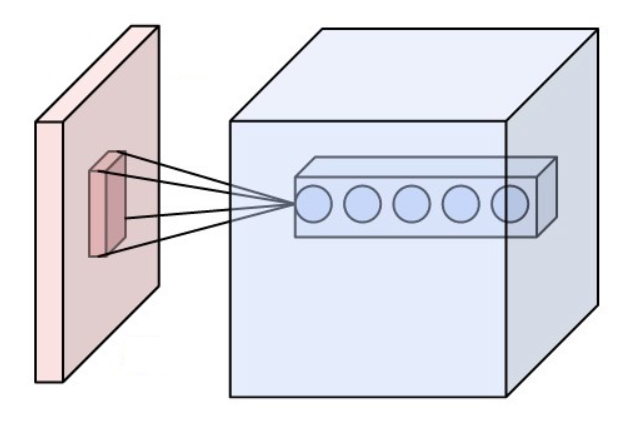
\includegraphics[width=0.6\textwidth]{gfx/conv-layer-1}
  \end{center}
  \caption{
    Stack of neurons applying different feature detections within a convolutional layer on the same perceptual region \cite{Aphex342015}.
  }
  \label{fig:sec:theory:convnets:conv-layer-1}
\end{figure}

\paragraph{Local receptive fields}
The term \emph{receptive field} is borrowed from the literature of neuroscience and it refers to an area of the body surface that triggers a neurological response in the presence of stimuli \cite{Sherrington1906,Alonso2008}.
In the context of convolution networks, receptive field refers to a region of the visual input, represented by an image, that is connected with one or several neurons that will react to it and is commonly called \emph{filter}.
Using local receptive fields means that neurons in the network will not react to the whole image but to a small region of it instead.
This ensures neurons will extract first the most basic visual features such as edges, end-points, or corners.
In subsequent layers, from those elementary visual features, neurons will then extract progressively higher-order features like shapes, textures, faces, objects, or scenes.
Such architecture allows effectively taking into account the spatial correlation existing in images.
Within a layer, several neurons performing different feature detections can be stacked to receive the input from the perceptive field as depicted in Figure~\ref{fig:sec:theory:convnets:conv-layer-1}.

\paragraph{Shared weights}
Layers in CNNs are organized in several slices, each of them containing neurons that detect the same feature but in different regions of the image and each slice detecting different features.
This operation is equivalent to a convolution in image processing, a sliding window that applies a transformation to the original image, and that is where CNNs receive their name.
The sliding window is called kernel, filter, or mask, and it is an image transformation matrix, usually small, that performs the weighted sum over a set of pixels of the original image, as shown in Figure~\ref{fig:sec:theory:covnets:kernel}.
In this analogy, the kernel of the convolution is the filter applied by the slice over the input, represented by \emph{weights shared} by all its neurons, being this what makes feature recognition robust against translations in the image.
The output of the convolution is referred to as \emph{feature map}, and all feature maps produced by a convolutional layer together become the input for the next layer, usually called \emph{volume} since it has height, width, and depth.
The height and width are proportional to the size of the original image, whereas the depth is equal to the number of slices in the layer.
Such architecture is depicted in Figure~\ref{fig:sec:theory:conv-layer-2}.

\begin{figure}[t]
  \begin{center}
    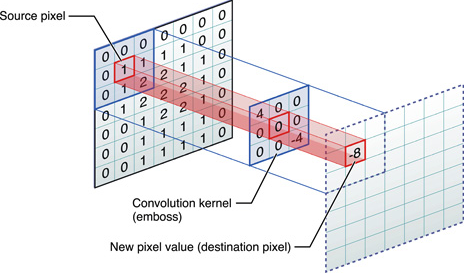
\includegraphics[width=0.5\textwidth]{gfx/kernel}
  \end{center}
  \caption{Convolutional kernel \cite{Apple}.
    The kernel gets centered on the source pixel and the convolution takes into account nearby pixels transforming the source pixel value.
    The convolution operation is a weighted sum of the source pixel with its nearby pixels. In this case:\\
    $(0\cdot4)+(0\cdot0)+(0\cdot0)
     +(0\cdot0)+(1\cdot0)+(1\cdot0)
     +(0\cdot0)+(1\cdot0)+(2\cdot-4) = -8$
  }
  \label{fig:sec:theory:covnets:kernel}
\end{figure}

\begin{figure}[t]
  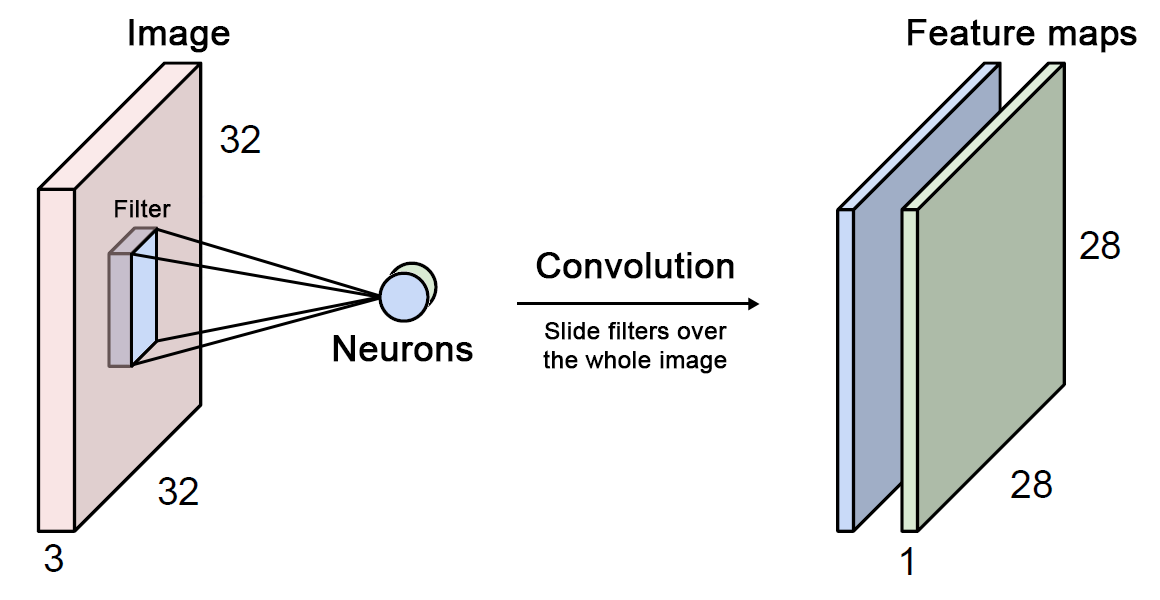
\includegraphics[width=\textwidth]{gfx/conv-layer-2}
  \caption{
    Anatomy of a convolutional layer and its output \cite{Guerzhoy2016}.
    On the left, the representation of an image of ${32}\times{32}$ pixels with $3$ color channels (\emph{RGB}).
    Neurons apply different filters of size ${5}\times{5}\times{3}$ in a particular region of the image.
    Together, all neurons applying the same filter within a layer produce what we call a feature map, resulting in as many as different filters are applied on the input.
    On the right, all produced feature maps combined become the input to the next layer as a ``new image'' of size ${28}\times{28}\times{N}$, being $N$ the number of filters in the layer.
  }
  \label{fig:sec:theory:conv-layer-2}
\end{figure}

\paragraph{Subsampling}
In the process of detecting higher-order features throughout subsequent layers of the network, the exact absolute position of detected features in feature maps is pretty much irrelevant compared to the relative position between them.
For instance, the pattern that describes the number $7$ is an endpoint in the upper left area of a horizontal segment, a corner in the upper right area, and an endpoint at the bottom of a vertical segment.
Still, small variations in the input may cause the pattern not to be detected because the features will not completely match the filter.
To make the network more robust against variations, the sensitivity of the convolutional layers has to be reduced.
This is effectively accomplished by reducing the resolution of the feature maps through non-linear \emph{subsampling} with pooling layers.
$Max$ is normally used as the non-linear function, giving the name of the subsampling operation \emph{max-pooling}, but it is not limited to it, as we will see in Chapter~\ref{chap:system}.
A pooling layer takes as input a volume of feature maps and, usually, has a non-overlapping filter of size ${2}\times{2}$ that gets applied on each one of the feature maps individually, as can be appreciated in Figure~\ref{fig:sec:theory:convnets:pooling}.
More specifically, the filter summarizes the feature map by performing max-pooling over its ${2}\times{2}$ regions and producing a single value for each, being this a size reduction of $75\%$.
It is important to note that this reduction applies only to the height and width of the original input since the depth refers to the number of feature maps and these are preserved.

\begin{figure}[t]
  \begin{subfigure}[b]{0.35\textwidth}
    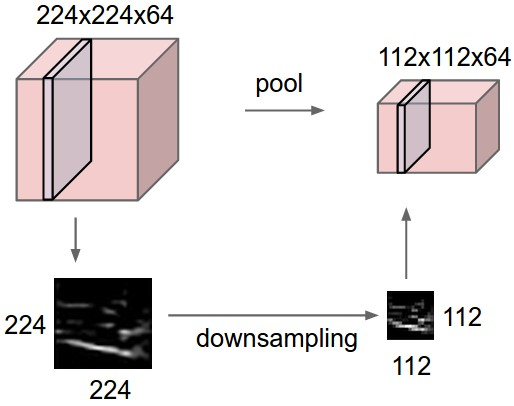
\includegraphics[width=\textwidth]{gfx/pool}
    \caption{General pooling}
    \label{fig:sec:theory:convnets:pooling:general}
  \end{subfigure}
  \hfill
  \begin{subfigure}[b]{0.55\textwidth}
    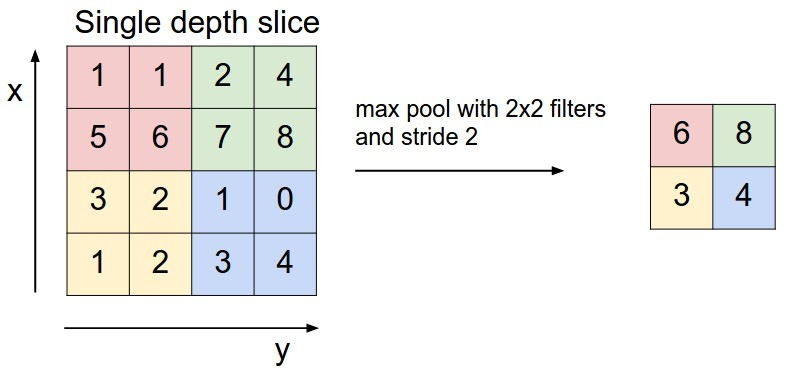
\includegraphics[width=\textwidth]{gfx/maxpool}
    \caption{Max-pooling}
    \label{fig:sec:theory:convnets:pooling:max}
  \end{subfigure}
  \caption{
    Overview of a pooling layer.
    On the left, the input and output of a pooling layer reducing only the height and width of the volume \cite{Karpathy}.
    On the right, a single feature map of the input volume being subsampled by non-overlapping ${2}\times{2}$ max-pooling \cite{Karpathya}.
  }
  \label{fig:sec:theory:convnets:pooling}
\end{figure}


\subsection{Architecture}
\label{sub:theory:convnets:achitecture}

While discussing the properties of CNNs, we introduced two of their building blocks: convolutional layers and pooling layers.
These alone are not enough to use CNNs for object recognition tasks since feature extraction is not the same as classification.
Let us have a look at how they fit in the big picture and the rest of the building blocks.

In Figure~\ref{fig:sec:theory:convnet} we present the typical configuration of a complete convolutional network.
We can see convolutional layers are alternated with pooling layers and ultimately fed into a fully-connected network.
Whereas convolutional layers generally increase the amount of feature maps making intermediate representations richer, pooling layers reduce their spatial resolution keeping the amount of parameters low and thus limiting overfitting.
After several convolutional-pooling layers, one final step is a fully-connected layer, where the classification finally takes place.
Optionally, normalization layers can be present after convolutional and pooling layers to increase the learning rate of the network.
During the learning process, the output of the classification at the end of the fully-connected layers is passed to a loss function that calculates the error of the prediction over a training sample.

\paragraph{Fully-connected layers}
The fully-connected layers is essentially a conventional fully-connected neural network only that we feed it with a set of feature maps produced by the convolutional layers, a highly-abstracted and rich representation of the original image at that point.
That means the data is much less noisy than raw pixels, so overfitting happens to a much lesser degree than what we discussed in \autoref{sec:theory:mlffnn:overfitting}.
Classification in the last layer is performed in the same fashion as we saw in \autoref{fig:sec:theory:mlffnn}, typically implemented as a $softmax$ layer that restricts the output to real values between 0 and 1, which summed add up to 1, representing the probability of the input belonging to the different classes.

\begin{figure}[t]
  \begin{center}
    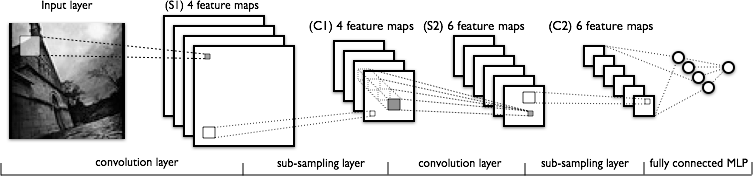
\includegraphics[width=\textwidth]{gfx/conv-network}
  \end{center}
  \caption{
    LeNet typical architecture \cite{Lisa2010}.
    On the left, there is an image (input layer).
    The image gets processed by a convolutional layer that extracts 4 elementary features producing 4 feature maps (S1).
    A pooling layer reduces the dimensionality while maintaining the same amount of feature maps (C1).
    Next, another convolutional layer extracts 6 higher-order features from the 4 feature maps (C2).
    Again, another pooling layer reduces the resolution of the 6 feature maps (S2).
    Finally, a fully-connected network takes the 6 feature maps and performs classification over them.
  }
  \label{fig:sec:theory:convnet}
\end{figure}

\paragraph{Normalization layers}
Additionally to these fundamental layers, normalization layers have been used as well, commonly referred to as \emph{Rectified Linear Units} or just \emph{ReLU}.
They simply use non-saturating activation functions like $max$ where the range is $[0,\infty]$, opposed to saturating activation functions like sigmoid where range $[0,1]$ to speed up the training phase \cite{Krizhevsky2012,Nair2010}.
The idea behind using non-saturating activation functions is minimizing the effects of the \emph{vanishing gradient problem} \cite{Socher2015}.
The vanishing gradient problem is a phenomenon in backpropagation that happens when weights adjust too slow on the first layers of very deep networks.
In them, the error contribution of each neuron in the initial layers will be very low and the saturating functions limit unnecessarily how much the weight can be adjusted.
Normalization layers, however, are falling out of use since it has been proved their contribution to the final result is very small and introduces new problems \cite{Lo2015}.

Summarizing, CNNs are mainly composed of convolutional layers, pooling layers, normalization layers and fully-connected layers.
Convolutional layers detect features in the input.
Pooling layers reduce the dimensionality of feature maps produced by convolutional layers.
Optionally, normalization layers magnify the non-linear properties of data to speed up learning.
Finally, fully-connected layers perform classification like we saw in \autoref{sec:theory:mlffnn}.


\subsection{Hyperparameters}
\label{sub:theory:convnets:achitecture}

In the next chapters, we will be looking at some already trained CNNs for image recognition.
Before we move on here is a quick recap of the architectural parameters that we will be talking about.

\paragraph{Convolutional input}
The shape of the receptive field in a convolutional layer.
It determines the local connectivity of neurons of the layer with neurons of the previous one.
It is normally larger in the first layer and it decreases for subsequent ones as the resolution decreases.
In image recognition tasks, it is common to range from $12x12$ to $15x15$ in the first layer.

\paragraph{Convolutional output}
The spatial arrangement of the output volume from a convolutional layer, which comes defined by \emph{depth}, \emph{stride}, and \emph{zero-padding}.
Depth represents how many neurons are connected to the same receptive field, each one applying a different filter.
It represents how many feature maps are produced as seen in \autoref{fig:sec:theory:convnets:conv-layer-1}.
Looking again at how convolution actually happens in \autoref{fig:sec:theory:covnets:kernel} will help to understand stride and zero-padding.
Stride defines how many units of separation the receptive field moves in the convolution operation and it represents the neuron density loss with respect to the previous layer.
With stride 1 there will be no ``gaps'' between neurons and their receptive field will be highly overlapped.
As stride goes up more ``gaps'' will appear, reducing the resolution of the output and making neurons' receptive field less overlapped.
Lastly, as seen in the convolution operation, the resolution of the result is smaller than the original on the edges.
Zero-padding is used to pad the output volume with zeros when maintaining the same resolution is required.

\paragraph{Pooling filter}
Shape of the filter in pooling layers, defined by height, width, and stride.
Usually $2x2$ filter with stride 2 are used, as in the example depicted in \autoref{fig:sec:theory:convnets:pooling:max}.
Stride is set to 2 so that the filters do not overlap.
